\documentclass[10pt]{beamer}
\usetheme[
%%% option passed to the outer theme
%    progressstyle=fixedCircCnt,   % fixedCircCnt, movingCircCnt (moving is deault)
  ]{Feather}
  
% If you want to change the colors of the various elements in the theme, edit and uncomment the following lines

% Change the bar colors:
%\setbeamercolor{Feather}{fg=red!20,bg=red}

% Change the color of the structural elements:
%\setbeamercolor{structure}{fg=red}

% Change the frame title text color:
%\setbeamercolor{frametitle}{fg=blue}

% Change the normal text color background:
%\setbeamercolor{normal text}{fg=black,bg=gray!10}

%-------------------------------------------------------
% INCLUDE PACKAGES
%-------------------------------------------------------
%\usepackage{xepersian}
%\settextfont[Scale=1]{IRNazanin}

\usepackage[utf8]{inputenc}
\usepackage[english]{babel}
\usepackage[T1]{fontenc}
\usepackage{helvet}
\usepackage{textpos}

\usepackage{amsmath}
\usepackage{hyperref}
\usepackage[]{algorithm2e}
%-------------------------------------------------------
% DEFFINING AND REDEFINING COMMANDS
%-------------------------------------------------------

% colored hyperlinks
\newcommand{\chref}[2]{
  \href{#1}{{\usebeamercolor[bg]{Feather}#2}}
}

%-------------------------------------------------------
% INFORMATION IN THE TITLE PAGE
%-------------------------------------------------------

\title[] % [] is optional - is placed on the bottom of the sidebar on every slide
{ % is placed on the title page
      \textbf{A Shape Constrained Parametric Active Contour Model For Breast Contour Detection\\}
}

%\subtitle[A Numerical Investigation Of Breast Compression]
%{
%      \textbf{Lesion Modeling}
%}

\author[S. Zarrin pour]
{      S. Zarrin pour \\
      {
      	\ttfamily sa.zarrinpour@iasbs.ac.ir\\
      	samim56b@gmail.com
  	  }
}

% logo of my university

\institute[]
{
	
      Mathematics Department, Institute for Advance Studies in Basic Sciences\\
      
      
  
  %there must be an empty line above this line - otherwise some unwanted space is added between the university and the country (I do not know why;( )
}

\date{\today \\ \vspace*{0.25cm}\hspace*{0cm}
\includegraphics[height=.5cm]{Feathergraphics/IASBSLOGO.png}}

%-------------------------------------------------------
% THE BODY OF THE PRESENTATION
%-------------------------------------------------------

\begin{document}

%-------------------------------------------------------
% THE TITLEPAGE
%-------------------------------------------------------

{\1% % this is the name of the PDF file for the background
\begin{frame}[plain,noframenumbering] % the plain option removes the header from the title page, noframenumbering removes the numbering of this frame only
  \titlepage % call the title page information from above
\end{frame}}

\addtobeamertemplate{frametitle}{}{%
	\begin{textblock*}{100mm}(.85\textwidth,6.5cm)
		
\includegraphics[height=.75cm,width=2.5cm]{Feathergraphics/IASBSLOGO.png}
\end{textblock*}}

\begin{frame}{Outline}{}
\tableofcontents
\end{frame}

%-------------------------------------------------------
%-------------------------------------------------------
\section{Breast Cancer Statistics}
\begin{frame}{Introduction}{Breast Cancer Statistics} 
%-------------------------------------------------------
Breast Cancer (C50), European Age-Standardised Mortality Rates per 100,000 Population, Females, UK, 1971-2016
\begin{figure}[t]
	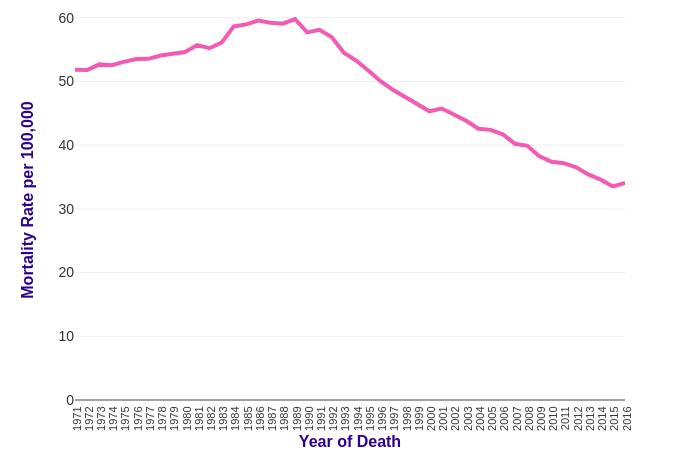
\includegraphics[width=8cm]{Feathergraphics/plot1}
	\centering
\end{figure}
\end{frame}

\begin{frame}{Introduction}{Breast Cancer Statistics} 
%-------------------------------------------------------
Breast Cancer (C50), European Age-Standardised Mortality Rates per 100,000 Population, Males, UK, 1971-2016
\begin{figure}[t]
	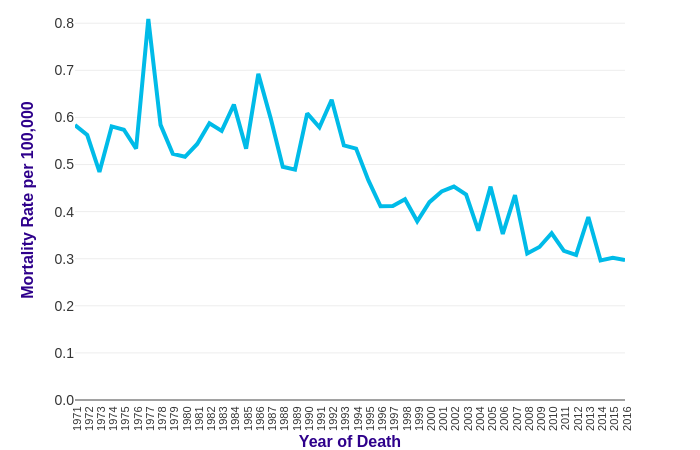
\includegraphics[width=8cm]{Feathergraphics/plot2}
	\centering
\end{figure}
\end{frame}
\section{Breast Reconstruction}
\begin{frame}{Introduction}{Breast Reconstruction} 
%-------------------------------------------------------
\begin{block}{}
	Importance
	\begin{itemize}
		\item {\tt Restoring breast cancer survivors' quality of life}
		\item {\tt Save patient from Confusion}
	\end{itemize}
\end{block}
\end{frame}


\begin{frame}{Introduction}{Breast Reconstruction} 
%-------------------------------------------------------
Previous algorithm limitations
\begin{itemize}
	\item<2- > strong gradient changes like nipple/areola 
	\item<3- > not validated with clinical photographs 
\end{itemize}
\end{frame}
\section{Proposed Approach}
\begin{frame}{Proposed Approach}{Active contour} 
%-------------------------------------------------------
\begin{block}{Defenition}
	An active contour is a parametric curve $v(s) = [x(s) ,y(s)]^T , s \in [0,1]$ that evolves to
	minimize the following energy functional 
	
	\vspace{5pt}
	\begin{gather} 
	\int_{0}^{1} \Big[\frac{1}{2} (w_{1}v_{s}(s) + w_{2}v_{ss}(s))^2 + E_{ext} \Big] \, ds	
	\end{gather}
	\vspace{5pt}
	\\where \\
	\begin{itemize}
		\item $v_{s}(s)$ \em\& $v_{ss}(s)$ are first and second derivative
		\item $w_{1} $ \em\& $w_{2}$ are associated weights to continuity and curvature of the contour
		\item $E_{ext}$ is the external forces that influence the curve evolution.
\end{itemize}
\end{block}
\end{frame}

\begin{frame}{Proposed Approach}{$E_{ext}$} 
%-------------------------------------------------------
\begin{itemize}
	\item an image with oriented structure enhanced
	\item obtained by a quadrature pair comprized of the steerable forth derivative of a 2D gaussian and its Hilbert transform
	\item embeded within the VFC framework to make $E_{ext}$ robust to noise
\end{itemize}
\end{frame}

\begin{frame}{Proposed Approach}{Shape Constraint} 
%-------------------------------------------------------
\begin{itemize}
	\item to incorporate the prior knowledge:
	$F_{shape}=(V(s)-v_{c}(s))^2 ,s \in [0,1]$ ,where
	\begin{gather}
	\mathbf{v_{c}(s)} :=
	\begin{pmatrix}
	\cos(\theta) & -\sin(\theta) \\
	\sin(\theta) & \cos(\theta)
	\end{pmatrix}
	\begin{pmatrix}
	\alpha \cdot 2(s-1)+b \\
	-\alpha \cosh(2(s-1))+c
	\end{pmatrix} 
	\end{gather}
	represents the rotated catenary curve which captures the overal curvature of the breast contour reliably.
	\item to prevent the contour from evolving towards a trivial local optima:\\
	$F_{baloon}\mathrel{\mathop:}=$  the unit normal vector of each vertex in the active contour
		  
\end{itemize}
\end{frame}

\begin{frame}{Proposed Approach}{Shape Constraint} 
%-------------------------------------------------------
The resulting Euler-Lagrange equation To minimize energy functional $E$ is :
\begin{gather}
w_{1}v_{ss}(s)-w_{2}v_{sss}(s)-\nabla E{ext}(v(s))-\lambda F_{shape}+\tau F_{balloon} = 0 
\end{gather}
which represented as $F_{int}+F_{ext}=0$ where $F_{int}$ is the internal forces to retain the continuity and $F_{ext}$ is the external force needed to attract the contour to the breast contour.
\end{frame}

\begin{frame}{Proposed Approach}{Shape Constraint}
to solve later equation the contour $v(s)$ is considered as a function of time $t$ and the steady state solution of it can be found using the gradient descent equation as follows
\begin{gather}
\frac{\partial v(s,t)}{\partial t} = F_{int}(v(s,t)) + F_{ext}(v(s,t)) 
\end{gather}
the initial value is defined as $v(s,0)=v_{c}(s,a_{0},b_{0},c_{0},\theta_{0})$ as an approximate to the breast contour.
\end{frame}

\begin{frame}{Proposed Approach}{Numerical Implementation} 
%-------------------------------------------------------
Initialization
\begin{itemize}
	\item let $S_{p}=[w_{1},w_{2},\lambda,\tau]$ denotes the static parameter set and let $S_{p} = [0.05, 0.15, 0.1, 0.2]$
	\item let $D_{p}=[a, b, c, \theta]$ denotes the dynamic parameters set.
	\item let $[a,\theta]$ be [70, 20] for for the patient's right breast contour and [70, -20] for patient's left breast contour
	\item the initial values for [b,c] will computed from the location of \em Anterior Axilliary Point \textbf{(AAP)} so one end of the active contour will be located in \textbf{AAP}
\end{itemize}
\end{frame}

\begin{frame}{Proposed Approach}{Numerical Implementation} 
%-------------------------------------------------------
the location of \textbf{AAP}
\begin{figure}[t]
	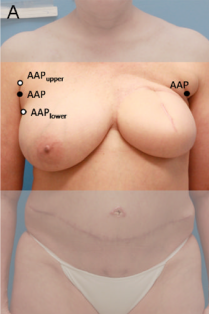
\includegraphics[width=4cm]{Feathergraphics/fig1A}
	\centering
\end{figure}
\end{frame}

\begin{frame}{Proposed Approach}{Numerical Implementation} 
%-------------------------------------------------------
\begin{algorithm}[H]
	\KwData{$S_{p}, D_{p}$}
	\KwResult{$v_{s}$}
	%initialization\;
	\While{$\sum_{i} |v(i,t)-v(i,t-1)| <\lambda$}{
		Update $v(i,t)$ by solving (4) \;
		Update $[a,b,c,\theta]$ from $v(i,t)$ by solving (2) in least square sence \;
		%\eIf{understand}{
		%	go to next section\;
		%	current section becomes this one\;
		%}{
		%	go back to the beginning of current section\;
		%}
	}
	\caption{computing active contour}
\end{algorithm}
\end{frame}
%-------------------------------------------------------
\section{Results}

\begin{frame}{Results}{compare with balloon model} 
%-------------------------------------------------------
traditional balloon model wthout shape constrained (B) \textbf{VS} proposed approach (C)
\begin{figure}[t]
	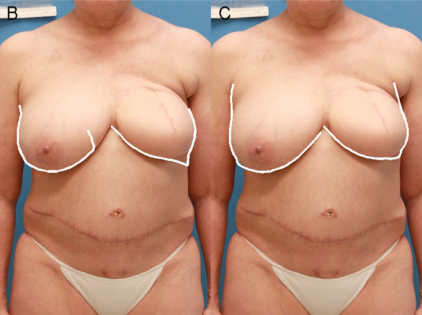
\includegraphics[width=6cm]{Feathergraphics/fig1BC}
	\centering
\end{figure}
\end{frame}

\begin{frame}{Results}{success cases} 
%-------------------------------------------------------
Example of success cases
\begin{figure}[t]
	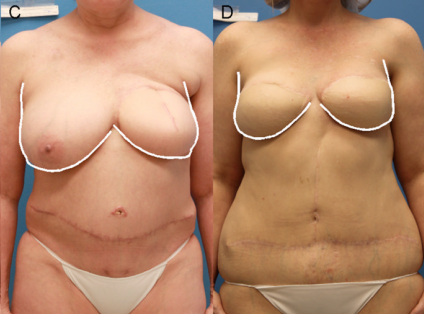
\includegraphics[width=6cm]{Feathergraphics/fig1CD}
\end{figure}
\end{frame}

\begin{frame}{Results}{failed cases} 
%-------------------------------------------------------
Example of failure cases
\begin{figure}[t]
	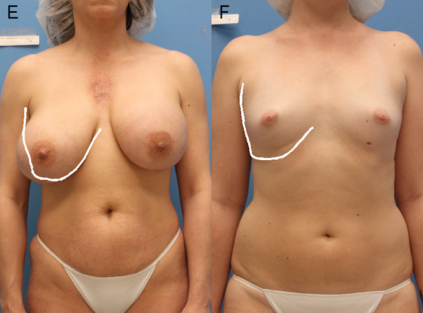
\includegraphics[width=6cm]{Feathergraphics/fig1EF}
	\centering
\end{figure}
\end{frame}

\section{Q\em\&A}
\begin{frame}{Q\em\&A}{} 
%-------------------------------------------------------
\textbf{"Ask, and it shall be given you!"}\centering\\
\em Matthew 7:7
\end{frame}
\section{References}
\begin{frame}{References}{} 
%-------------------------------------------------------
\begin{itemize}
	\item\href{https://www.cancerresearchuk.org/health-professional/cancer-statistics/statistics-by-cancer-type/breast-cancer/mortality}{https://www.cancerresearchuk.org}
	\item Lee, J., Muralidhar, G. S., Reece, G. P., \& Markey, M. K. (2012). A shape constrained parametric active contour model for breast contour detection. In Conference proceedings:... Annual International Conference of the IEEE Engineering in Medicine and Biology Society. IEEE Engineering in Medicine and Biology Society. Conference (Vol. 2012, p. 4450). NIH Public Access.
\end{itemize}
\end{frame}


%
{\1
\begin{frame}[plain,noframenumbering]

  \finalpage{Thank you for your attention.}
\end{frame}}

\end{document}